\documentclass[preprint, review, 12pt]{elsarticle}

\usepackage{lineno,hyperref}
\usepackage{amssymb}
\usepackage{url}
\usepackage{paralist}
\usepackage{booktabs}
\usepackage{colortbl}
\usepackage{gensymb}
\usepackage{soul}

\definecolor{DarkRow}{rgb}{0.9, 0.9, 0.9}
\modulolinenumbers[5]

\journal{Energy}

%%%%%%%%%%%%%%%%%%%%%%%
%% Elsevier bibliography styles
%%%%%%%%%%%%%%%%%%%%%%%
%% To change the style, put a % in front of the second line of the current style and
%% remove the % from the second line of the style you would like to use.
%%%%%%%%%%%%%%%%%%%%%%%

%% Numbered
%\bibliographystyle{model1-num-names}

%% Numbered without titles
%\bibliographystyle{model1a-num-names}

%% Harvard
%\bibliographystyle{model2-names.bst}\biboptions{authoryear}

%% Vancouver numbered
%\usepackage{numcompress}\bibliographystyle{model3-num-names}

%% Vancouver name/year
%\usepackage{numcompress}\bibliographystyle{model4-names}\biboptions{authoryear}

%% APA style
%\bibliographystyle{model5-names}\biboptions{authoryear}

%% AMA style
%\usepackage{numcompress}\bibliographystyle{model6-num-names}

%% `Elsevier LaTeX' style
\bibliographystyle{elsarticle-num}
%%%%%%%%%%%%%%%%%%%%%%%

\begin{document}

\begin{frontmatter}

\title{Scalable Tuning of Building Models to Hourly Data}

\author[atr:garrett]{Aaron Garrett}
\author[atr:new]{Joshua New\corref{cor}}
\cortext[cor]{Corresponding author at Oak Ridge National Laboratory; \emph{Email address}: newjr@ornl.gov}

\address[atr:garrett]{Mathematical, Computing, and Information Sciences, Jacksonville State University, Jacksonville, AL, USA}
\address[atr:new]{Oak Ridge National Laboratory, Oak Ridge, TN, USA}


\begin{abstract}
Energy models of existing buildings are unreliable unless calibrated so they correlate well with actual energy usage. Manual tuning requires a skilled professional, is prohibitively expensive for small projects, imperfect, non-repeatable, non-transferable, and not scalable to the dozens of sensor channels that smart meters, smart appliances, and cheap/ubiquitous sensors are beginning to make available today. A scalable, automated methodology is needed to quickly and intelligently calibrate building energy models to all available data, increase the usefulness of those models, and facilitate speed-and-scale penetration of simulation-based capabilities into the marketplace for actualized energy savings. The ``Autotune'' project is a novel, model-agnostic methodology which leverages supercomputing, large simulation ensembles, and big data mining with multiple machine learning algorithms to allow automatic calibration of simulations that match measured experimental data in a way that is deployable on commodity hardware. This paper shares several methodologies employed to reduce the combinatorial complexity to a computationally tractable search problem for hundreds of input parameters. Accuracy metrics are provided which quantify model error to measured data for either monthly or hourly electrical usage from a highly-instrumented, emulated-occupancy research home.
\end{abstract}

\begin{keyword}
Autotune, EnergyPlus, calibration, optimization, evolutionary computation
\end{keyword}

\end{frontmatter}

%\linenumbers

\section{Introduction}
\label{sec:introduction}
Sustainability, with its connections to energy and climate change, is perhaps the defining challenge of our time. With only 4.4\% of the world's population, the United States (U.S.) consumes 19\% of the world's primary energy production. The largest sector of energy consumption in the U.S. is buildings, which consumed 41\% of national primary energy production in 2010; 19\% was consumed by approximately 4.7 million commercial buildings and 22\% by 114 million residential buildings \cite{cit:doe2012a}. Building energy model creation and simulation can provide many functions, but is often fiscally infeasible for all but the largest of projects due to the time required to create a model of an existing building and calibrate it to measured data. The U.S. Department of Energy's (DOE) Building Technology Office (BTO) is assisting development of several Emerging Technology (ET) applications to significantly reduce cost and drive simulation-informed actualized energy savings into existing light commercial and residential buildings in order to meet the nation’s overarching goal to reduce building energy use 50\% by 2030 compared to a 2010 baseline.

There are many simulation-based analysis tools available which are used to project how specific policies or retrofit packages would maximize return-on-investment with subsidies through federal, state, local, and utility tax incentives, rebates, and loan programs. Resolving well-known issues such as principle-agent, first cost, and cost/performance trade-offs as well as maximizing financial metrics such as net present value, rate of return, cost of conserved energy, and simple pay-back fall within the domain of these tools. Like all software tools, such analysis suffers from ``garbage in, garbage out'' (GIGO). This is complicated by the fact that unlike cars or planes built to a strict engineering specification, buildings are currently based on one-off designs and constructed in the field. These buildings can last decades or hundreds of years and rarely does any sensor data exist beyond utility bill data. In such cases, optimal retrofit packages and similar analysis are calculated for a fictitious building and necessarily yield suboptimal results. A central challenge in the domain of building energy efficiency is being able to realistically and cost-effectively model existing buildings. Even coarse models are useful to determine incremental energy conservation measure (ECM) changes/impact to whole-building energy consumption. That usefulness is dramatically increased for existing buildings where existing data can be used to calibrate the energy model. However, differences from actual monthly utility bills on the order of 24\%-97\% \cite{cit:earthadvantage2009,cit:roberts2012} are currently common. Many measurement and verification (M\&V) protocols specify a required accuracy to be a legally useful model. Most large organizations use ASHRAE Guideline 14's 5.3.2.4.f requirements which specifies coefficient of variance for root mean squared error CV(RMSE) \textless 15\% or 30\% and normalized mean bias error NMBE \textless 5\% or 10\% for calibrating to monthly or hourly data, respectively \cite{cit:ashrae2002}.

There are several simulation engines, and tools which leverage those simulation engines, that are actively supported by DOE \cite{cit:doetools2012}. DOE’s flagship simulation engine is currently EnergyPlus \cite{cit:energyplus} and has been supported with over \$65 million since 1995. OpenStudio \cite{cit:nrel2012} now serves as the primary middleware between simulation engines and analysis tool applications. High-level graphical interfaces and low-level, text-based files allow a user to provide information that fully describes a given building and from which EnergyPlus can calculate detailed heat flow and energy usage information for the building. The number and instances of these input parameters are extensive, highly variable in their combinatorial effects, and their sensitivities are not yet fully explored. This relegates simulation calibration to an ``art'' for which only a few hundred people have qualified for ASHRAE's building energy modeling professional certification. It is unrealistic to expect even an advanced user to be capable of providing accurate values for each of the approximately 3,000 parameters expected by EnergyPlus for the average building. To mitigate such issues, users often use a reference or template building already in their preferred tool that is similar to their own as a default point for parameter values. These values are then ``corrected'' to more closely match the actual building under consideration depending on the level of information available such as those specified by an ASHRAE level 1, 2, or 3 audit. In addition, average material properties are typically used from the ASHRAE Handbook of Fundamentals (HoF) which is now beginning to include significant variances in material properties identified from controlled laboratory tests \cite{cit:ashrae2013}.

As the variance of material properties increase, as the number of different systems, envelopes, equipment, components, and materials become more complicated and diverse, and as energy simulation modeling algorithms evolve to more thoroughly model existing systems and capture new equipment technologies, there will be a growing need to mitigate this increase in complexity by relying on cost-effective, intelligent algorithms to calibrate building energy models in a way that uses as much data as available. The Autotune project \cite{cit:new2012} aims to solve this need with an automated process and has previously demonstrated calibration results for envelope parameters using monthly utility data \cite{cit:garrett2013}. This paper extends that work by discussing the scalable methodologies used to tune a building energy model's 100+ envelope parameters to whole-building hourly electrical usage data.

\section{Background}
\label{sec:background}
This section discusses a quick survey of Autotune project results, previous surveys of simulation accuracy for multiple simulation engines, the causes for this inaccuracy, background on the process of calibrating energy models to measured data, the computational complexity involved in solving the calibration problem, and considerations in the selection of evolutionary computation methodologies employed for automated calibration.

\subsection{Autotune Background}
The Autotune project has used 269+ channels of 15-minute sensor data from a robotically emulated-occupancy ZEBRAlliance \cite{cit:miller2012,cit:biswas2012} 2800 ft$^2$ research home. Parametric ensemble models of this building were simulated using high performance computing (HPC) resources. Titan, currently the world’s second fastest supercomputer, allowed the use of 131,072 cores to calculate 524,288 simulations and write 44 TB of data to disk in 68 minutes \cite{cit:sanyal2013a}. Some of the latest advances in web-oriented database storage were used to allow queryable simulations generated from varying 156 inputs and reporting 96 outputs at 15-minute resolution (35 MB per simulation) for 8 million EnergyPlus simulations \cite{cit:sanyal2013b}. Measured data can often be corrupt from uncalibrated sensors or missing data, so statistical techniques have been refined for autonomous quality assurance and gap-filling \cite{cit:castello2012}. Extensive big data mining was conducted through creation of an HPC-enabled suite of machine learning algorithms (MLSuite \cite{cit:edwards2013}) to generate agent-based encapsulation of knowledge for Autotune deployment on mobile devices. EnergyPlus was approximated with machine learning algorithms to reduce simulation runtime from 8 minutes to 3 seconds with minimal trade-off in accuracy for the processed building types \cite{cit:edwards2013}. The Autotune project, in an effort to promote open science, is making a portion of the 267 TB (26.9 trillion data points) of EnergyPlus simulation data freely available online\footnote{\url{http://autotune.roofcalc.com}}.

\subsection{Simulation Accuracy}
Despite the proliferating use of building energy tools via their integration with research and development (R\&D) initiatives, policies, tax structure, codes and standards, and product sales, there remain many concerns and shortcomings applicable to all simulation engines. The primary concern is typically the accuracy of the simulation engines for realistically modeling (via inputs) a virtual building such that it matches a real-world building. This is a well-established issue that has remained unresolved in the energy modeling community. A Home Energy Rating System (HERS) study in 1999 \cite{cit:pigg2001} using the REM/Rate
simulation engine for 2,300 homes in Wisconsin found that the median home's heating use, which accounts for 40\% of the average annual Wisconsin energy bill, is overestimated by 22\% with the worst 15\% median being off by 62\%. A 2008 pilot study \cite{cit:earthadvantage2009} found 190 Home Energy Saver, REM/Rate, and SIMPLE residential simulation models had 25.1\%--96.6\% error compared to actual monthly electrical energy usage. A recent 2012 study \cite{cit:roberts2012} found that for 859 residential models across Home Energy Saver, REM/Rate, and SIMPLE simulation engines had a mean absolute percent difference of 24\% from actual monthly electrical energy usage and 24\%--37\% from actual natural gas use for a sample size of 500 houses. It should be noted that all of these studies use comparisons to monthly utility bill data; the challenge of accurately matching hourly or 15-minute data for dozens of sub-metered data channels is significantly more difficult.

The challenge for simulation accuracy can be reduced to two primary issues: \begin{inparaenum}[1)]
\item a gap between the as-modeled and as-built structure and 
\item limitations of the modeling engine's capabilities. 
\end{inparaenum}
We will discuss each of these in detail.

\subsection{Common Errors with Simulation Inputs}
Gaps between as-modeled and as-built structures come in many sources with the fault being traceable to an inaccurate input file rather than the simulation engine itself. We have worked with building scientists and conducted sensitivity analysis to identify the most important input parameters.

Infiltration, the rate at which air and the energy in it flows through the building envelope (typically measured in cubic feet per minute per square ft), is not currently able to be cheaply tested despite being one of the most important factors for building energy efficiency. Blower-door tests can determine infiltration rate at a given pressure (usually 50 Pascals), but these are 1-time measurements that, in reality, experience significant variances as a function of other variables such as temperature, wind speed, and wind direction. As such, infiltration is often one of the first variables most energy modeling experts use to manually align a simulation model with actual data.

A second issue is the schedule for the building usage which includes number of occupants, times of occupancy, HVAC setpoints, operations schedule, and many other factors. These also constitute inputs to the simulation engine, but often specified in a separate EnergyPlus file for convenience. For many of these, cost-effective sensors simply do not exist or are not typically deployed in a building (especially data provided in a way to be easily leveraged by energy modelers). In many cases, estimates of occupancy schedules and relatively static setpoint temperatures are estimated and then used later to ``true-up'' the simulation to match whole-building data without regard to the accuracy of the actual HVAC thermostat setpoints.

A third component that modelers often do not use but which laboratory testing has exposed as a major contributor to model variance is material properties used within a building model. Most modelers typically use material properties from the ASHRAE Handbook of Fundamentals (HoF), which relates the average value of a physical property (e.g., roughness, conductivity, density, specific heat, thermal absorptance) for a given material (e.g., 5/8" gypsum board, cultured stone, 2-3/8" glass fiber insulation, 1/2" plywood, 2x6" wood studs) based on standard tests. Occasionally, materials ship from a manufacturer with labels that give more reliable estimates than the average values found in ASHRAE's HoF. However, laboratory-controlled hotbox testing of specific materials has shown significant variance in materials even from a single manufacturer. While many of these values are used to update the ASHRAE HoF's numbers over time, data has traditionally not been reported for variance but this is expected to change in future versions of the HoF. In such cases, energy modelers have very little reliable data to determine the precise values necessary for creating an accurate model of material properties for an individual building's construction.

A fourth gap is that energy modelers typically use building design, increasingly building information model (BIM) files, or similar documents for energy modeling, but craftsmanship influences how those designs are implemented (e.g. contractor neglects to put insulation in a corner wall). While several more gaps exist, it is important to note that most of these gaps remain due to the fact that current business models find saving relatively cheap energy does not provide enough incentive to justify the energy modeling expense. For example, a financial analysis of 26 Federal Energy Management Program (FEMP) Energy Service Company (ESCO) projects on commercial buildings showed that project development costs involving simulation ranged from 10--45\% of total cost for projects smaller than \$1 million. This enhanced risk prohibits financing for traditional, simulation-informed calibration and optimization of building retrofits for all but the largest building renovation projects.

\subsection{Common Errors with Simulation Algorithms}
Limitations of engine modeling capabilities are a well-understood and active area of involvement with funded development teams or active communities/ecosystems behind the most popular simulation engines and tools. It is common for there to be a backlog of hundreds of user requests involving inaccuracies of specific algorithms. Unlike the one-off use of a calibrated simulation model for a single building, there is sufficient market incentive and policy impact to be found in developing a capable software engine that can be applied to the entire building stock. Such engines are often used to inform policy decisions toward cost-effectively meet national energy goals. While several companies have developed simulation engines tied closely with their product line, an increasing number are either using co-simulation or swapping over to the large simulation engines like EnergyPlus. However, there are a few primary factors that may be considered in relation to inaccuracies of simulation engines.

First, most simulation engines are engineering models that attempt to model, through time and with some degree of fidelity, the underlying physics involved in energy consumption. As is necessary from such an approach, engineering algorithms are by necessity an approximation of reality (e.g., uses 1D heat transfer processes because 3D heat transfer would take too long to calculate). Some simulation engines allow selection of precision on an algorithmic level to allow customization for a particular area of interest. Statistical models show some promise, but are more useful in normative-based models for policy decisions rather than product-level or system-level modifications to a building. Second, there is a lag between the development of new, innovative technologies and the capabilities of accurately modeling it within a simulation engine. Only the most active simulation engine development teams are able to keep up with or foresee the need to model products, components, or systems of a building before they achieve a significant market share. As the codebase grows, the challenge of maintaining a software architecture that can accommodate new integrated technologies (which may impact several parts of a building) also grows in like manner. Third, virtually all known simulation engines are single-threaded with only recent attempts to leverage traditional multi-core and Graphical Processing Unit (GPU) computational hardware. Given the significantly different multi-threaded software development paradigms, there will be substantial challenges in being able to scale additional simulation capabilities without an increase in runtime for models that use those capabilities. Fourth, the computer itself is an approximation engine and is fundamentally limited with respect to the accuracy that it can provide in a unit of time for a given algorithm. For most simulation engine developments, the focus has been a reactive process of building something that is sufficient to meet some small fraction of the long list of needs expressed by the users.

The Autotune project's \cite{cit:new2012} goal is to create an automated process for tuning simulation inputs such that simulation output matches measured data. This repeatable, transferable, and scientifically rigorous process can address both inaccuracies in input as well as algorithm by 
\begin{inparaenum}[1)]
\item adapting a model to more closely match real-world data from the as-built structure and 
\item doing so in a way that accommodates inaccuracies in the underlying engineering
model.
\end{inparaenum}

\subsection{Tuning of Building Models}
While inaccurate models can be useful in comparative analysis, calibrated models are more useful and must often meet specific calibration criteria to be legally permitted for use in a specific context. To satisfy these requirements, modification of simulation algorithms can help address address the mismatch (often by working around limitations of a given simulation engine) remains one the most tractable methods used by experts. As previously mentioned, this tuning process has remained an ``art'' which even the practitioners most often do not enjoy. Informal interviews and surveys have indicated less than 3\% of people actually enjoy the tuning process and, instead, see it as a necessary and laborious process. These practitioners often indicate the use of infiltration and schedules (of many types) as the primary ``knobs'' by which to tune the simulation to measured data. As previously detailed, properties of the many materials alone provide hundreds more ``knobs.'' This means building model calibration is a severely under-determined problem with thousands of inputs that can be varied to match potentially only 12 data points, leading to questions as to the physical realism of the final ``tuned'' model from the very large number of valid models. As a starting point, this research paper will focus on the most important task of getting the thermal characteristics of the envelope right by tuning envelope properties in a way that matches electric consumption throughout the building.

It should come as no surprise that, in order to reduce the cost of business, the idea of self-calibrating energy models has been around for decades with initial attempts beginning around the early 1980s. Much of the motivations, history, different levels of thoroughness in calibration, and previous approaches (sensitivity analysis, reducing the number of simulations necessary, optimization methods, etc.) are expertly consolidated in ASHRAE report 1051-RP on the subject \cite{cit:reddy2006}. The Federal Energy Management Program (FEMP) also has rigorous Measurement and Validation (M\&V) guidelines \cite{cit:femp2008}.


\subsection{Computational Complexity}
The EnergyPlus whole-building energy simulation engine was consolidated from diverse involvement circa 1995 with functionality traceable back to DOE-2 and the U.S. Department of Energy's Building Loads Analysis and System Thermodynamics (BLAST) from the late 1970s \cite{cit:energyplus}. Its original design goals were to provide a more consistent software structure for development and modification, to allow third-party programs and components to easily interface with the core system, and to fully integrate the loads, systems, and plants into the simulation \cite{cit:energyplus}. The workflow for a building modeler using a system like EnergyPlus is to create a building's geometry using external software, layer it with detailed metrics encoding material properties, and add equipment currently or expected to be in the building, including anticipated operational schedules.

A typical residential building model in EnergyPlus has approximately 3,000 input parameters that must be specified. The search space in such a problem is extremely large. Even if each parameter were a simple binary value (e.g., a categorical whose values were \emph{yes} or \emph{no}), the search space for a 3000-parameter building would contain $2^{3000}$ possibilities, which is unfathomably larger than the number of atoms believed to exist in the observable universe (about $2^{270}$). This is a best-case scenario; the actual size of the search space is effectively infinite because many of the parameters are continuous-valued. For this study, we relied on several building simulation experts to identify 156 input parameters along with minimums and maximums within which they will be varied. Even with this simplification, to solve this problem with brute force would require Titan (currently the second fastest supercomputer in the world) more than $10^{28}$ lifetimes of the known universe (13.8 billion years) to calculate all the necessary EnergyPlus simulations to find the best model for a single residential building. Many of the experiments in this paper discuss algorithms and methods to find near-optimal models in a tractable amount of time on commodity hardware.

\subsection{Evolutionary Computation}
A common approach to such search problems, and one that has been successfully applied in previous building model tuning work \cite{cit:garrett2013}, is evolutionary computation (EC). Evolutionary computation \cite{cit:dejong1993,cit:spears1993,cit:fogel1994,cit:fogel2000} is a stochastic search algorithm that attempts to mimic biological evolution by maintaining a set of candidate solutions, referred to as a \emph{population}. Each candidate solutions is evaluated in order to determine its \emph{fitness}, which is a problem-dependent measure of how well it solves the problem \cite{cit:dejong2006}. In essence, the candidate solutions act as samples of the search space, and their fitness values provide an approximation of the gradient. However, unlike strict gradient-based techniques, an EC provides some (typically small) opportunity for less fit candidates to influence the search process, which helps the EC to avoid local optima \cite{cit:michalewicz2004}. 

Since evolutionary computation is a population-based search, it has a number of aspects that are inherently parallel. Most importantly for this work, each candidate in the population must be evaluated to determine its fitness, and the evaluation of one candidate is typically independent of the others. For expensive evaluation functions, the ability to determine the fitness values of an entire population simultaneously greatly increases the search efficiency. In addition to parallel evaluations, EC approaches called \emph{island models} \cite{cit:eiben2007} exist that maintain multiple populations with all performing parallel evolution. In many cases, each island (i.e., isolated population) is allowed to explore a different region of the search space, possibly in different ways. With most island models, there are mechanisms in place that allow candidate solutions to \emph{migrate} between islands (usually with low frequency), which allows information exchange between the populations.

In the context of this work, a candidate solution is a building with a chromosome represented by a list of building model parameters to be tuned. To evaluate a candidate solution, its corresponding EnergyPlus IDF model is constructed and passed to the EnergyPlus simulation engine, producing an entire set of output measures (e.g., heating/cooling loads). These output measures are then compared to actual measured data from the building. The resulting measure of accuracy is used as the fitness for the candidate solution.

The interaction among candidate solutions in the population drives the evolutionary process, and this interaction is defined in terms of \emph{evolutionary operators}. These operators determine how current solutions are recombined or modified to produce new solutions, as well as which solutions get to contribute information to the next generation. The particular evolutionary operators used in this work were heuristic crossover, Gaussian mutation, tournament selection, and generational replacement. Each of these operators is standard in the EC literature, and all were described previously in \cite{cit:garrett2013}.


\section{Methodology}
\label{sec:methodology}
Previous work \cite{cit:garrett2013} focused on tuning a building to monthly utility data. The work presented here takes a more ambitious approach by attempting to optimize the match between a model building and actual hourly electricity usage data. The reference building used in this work is house number 1 in the Wolf Creek subdivision (WC1), an Oak Ridge National Labs ZEBRAlliance experimental energy efficient home. This home has a plethora of energy-efficient technologies: 
\begin{inparaenum}[(1)]
\item standing seam metal roof with infrared reflective pigments to boost solar reflectance,
\item ENERGY STAR appliances, 
\item triple-pane low emittance Argon-filled windows, 
\item compact fluorescent lighting, 
\item horizontal ground loop installation that leverages foundation and utility excavations, 
\item high-efficiency water-to-air heat pump for space conditioning, 
\item high-efficiency water-to-water heat pump for hot water heating, 
\item an energy recovery ventilator for transferring heat and moisture between fresh incoming and outgoing air, and 
\item structurally insulated panel (SIP) walls filled with expanded polystyrene insulation.
\end{inparaenum}
For more information, the interested reader is referred to \cite{cit:miller2012,cit:biswas2012}. The home has been fitted with over 300 sensors that collected data at 15-minute timesteps using standard, wired-sensor data acquisition systems.

\subsection{Base Models}
The data, models, and accuracy metrics described in the remainder of this subsection are an extension of those previously reported in \cite{cit:garrett2013}. In the following experiments, two different model buildings are used. The first model, referred to here as the \emph{refined} model, was last modified on March 29, 2012. This model matches whole-building annual electric consumption exactly, but it has a sum of absolute errors (SAE) of 1,276.34 kWh for monthly and 6,242.04 kWh for hourly electrical data over the entire year. An earlier version of that same model was completed on July 28, 2010, and it is referred to here as the \emph{primitive} model. It has an SAE of 1,623.36 kWh for monthly and 8,113.69 kWh for hourly electrical data when summed for the entire year. These two baseline models are separated by approximately four person-months of effort (consisting of two months of laboratory material testing and two months manually tuning the input file) over the course of nearly two calendar years, with the refined model being the recipient of that effort.

\subsection{Tuning Parameters}
Only a subset of the real-valued parameters of the models, as specified by domain experts, was used as a part of the tuning process; the phrase ``tuning parameters'' will be used when referencing these variables. While all 156 tunable parameters provided through the project website\footnote{\url{http://bit.ly/autotune_parameters}} are too extensive to list here, a majority of the parameters were for building material properties such as thickness, conductivity, density, specific heat, thermal absorptance, solar absorptance, and visible absorptance for materials such as gypsum board, stone, concrete foundation wall, fiberglass insulation, metal roofing, plywood, insulation, gravel, oriented strand board (OSB), and cladding as well as U-factor, solar heat gain coefficient, and visible transmittance for window glazing systems. Other parameters include fraction of latent and radiant for equipment, radiant and visible for lighting, flow coefficients for HVAC, heating and cooling air supply temperatures, building orientation, infiltration, and several others. It should also be noted while these are individual line changes in an EnergyPlus IDF input file, several instances of each material, equipment, etc. may be used throughout a building. The Autotune system currently scales to tune any set of numerical parameters and can be customized for tuning only selected parameters in customizable ways. This allows calibration according to the needs of a particular use case or comparison to manual tuning efforts.

\subsection{Measured Data}
In 2010, the average U.S. residential building consumed enough energy to cost the homeowner \$2,201 \cite{cit:doe2012a}. An average of 44.7\% of the energy went to space heating and 9.2\% toward space cooling \cite{cit:doe2012b}, totaling 53.9\% for space conditioning. However, primarily because of differing costs for various fuel types \cite{cit:doe2012c}, 28.9\% of cost was for heating and 14.0\% for cooling, yielding 42.9\% and amounting to \$944/year for space conditioning. However, the energy-efficient HVAC in WC1 actually consumed \$472.62 for Jan. 1--Nov. 30, 2010. This 50\% cost reduction for an energy-efficient home may serve as a point of reference for the tuning results presented throughout the residential study.

For the all-electric WC1, the actual energy usage data for all HVAC equipment was reliably collected from January 1 through November 28, 2010 at which point a new set of test HVAC equipment was installed. Therefore, in all experiments reported, the ``yearly'' electrical usage (and, likewise, the ``full'' schedule) will always refer to the electrical usage from January 1 to November 28. The electrical usage in this work was calculated as the sum of all of the heating and cooling ideal loads for every time period (in kilowatt-hours).

\subsection{Tuning Accuracy}
In the following experiments, the primary metric used for measuring tuning accuracy is the sum of absolute errors (SAE)\footnote{The sum of absolute errors was chosen as the primary metric, rather than root mean squared error, for example, because of its ease of interpretation in terms of dollars difference.}. The SAE was calculated according to Equation~\ref{eq:sae}, where $M_i$ is the heating+cooling load of the model and $A_i$ is the heating+cooling load of the actual ZEBRAlliance WC1 building. This equation only contains $n=8016$ hours because actual data was not collected for December; this value is indicated as $SAE_{hour}$. One of the acceleration methods used is to tune on an abbreviated schedule of only four days (January 1, April 1, August 1, and November 1) before transitioning to a full year; use of this variant of the metric will be indicated as four-day SAE.

\begin{equation}
\label{eq:sae}
	SAE = \sum_{i=1}^{n}\left|M_i - A_i\right|
\end{equation}

One practical consideration in moving from monthly to hourly data is that failures and sensor drift are more prevalent and easily detectable. For this dataset, it was found that sensors failed to make a measurement in approximately 2\% of all measurements. In \cite{cit:garrett2013}, when dealing with error calculations, the failures were treated as 0 values in the summation because it was believed they would not significantly impact monthly usage. For hourly data, however, it makes a 4-fold larger difference, and it was decided to ignore any hour which contained at least one sensor failure (approximately 8\% of the data).

\subsection{Evolutionary Computation Parameters}
In the following experiments, we always use 1,024 fitness evaluations (EnergyPlus simulations compared to actual data) to allow comparison across experiments. These evaluations are organized into 16 individuals (building models) evolved over 64 generations, tournament selection with tournament size 4, generational replacement with weak elitism (one elite), heuristic crossover, and Gaussian mutation with a usage rate of 1.0 and a mutation rate of 10\% of the allowable range of each variable, unless otherwise specified. Because of the stochastic nature of this approach, results are shown for 8 independent trials.



\section{Experiments}
\label{sec:hourly}

\subsection{Experiment 1---Determining a Fitness Surrogate}
\label{sub:experiment1}
An annual EnergyPlus simulation for the WC1 reference building at one-hour time intervals (over 8,000 time periods) requires 8 minutes of runtime and cannot currently be efficiently parallelized. This type of fine-grained schedule leads to a much more exact, but computationally expensive, simulation. A four-day simulation has only 96 time periods of output data but can run in seconds. It was also previously established \cite{cit:garrett2013} that tuning on an abbreviated schedule of only four days (January 1, April 1, August 1, and November 1) was a defensible acceleration method for monthly data, and this experiment validates the same behavior for hourly data. We do this by establishing a correlation between the error rate of the four-day and full schedules, which requires a particular kind of sampling that spans from high to low error. An EC was used to minimize the error in the abbreviated schedule, and the hourly error in the four-day and full schedules of each created individual were measured and stored in order to determine their correlation. To ensure against statistical anomalies, the EC was run four different times with different initial populations each time.

The entire set of 1,024 individuals for each of the four trials is plotted in Figure~\ref{fig:hour-corr}. This plot compares the hourly sum of the absolute errors (SAE) between the candidate solutions and the actual energy usage, both for the four-day schedule and the full schedule, for each of the four independent trials. It is clear from the graph that there is a strong linear correlation between the electricity usage with the four-day schedule and that of the full schedule. More precisely, this correlation was 0.9697, 0.9704, 0.9472, and 0.9382 for each of the four trials, respectively. This can be seen in the first row of Table~\ref{tab:hour-corr}, which shows how the correlation changes as the data focuses more on the later generated samples (which would typically have lower SAE). So, as with previous results, the four-day abbreviated schedule appears to be an acceptable surrogate for the full schedule. It is an open, relevant, and interesting question as to which smallest subset of days provides the best correlation to full-schedule error.

\begin{figure}[tbp]
\centering
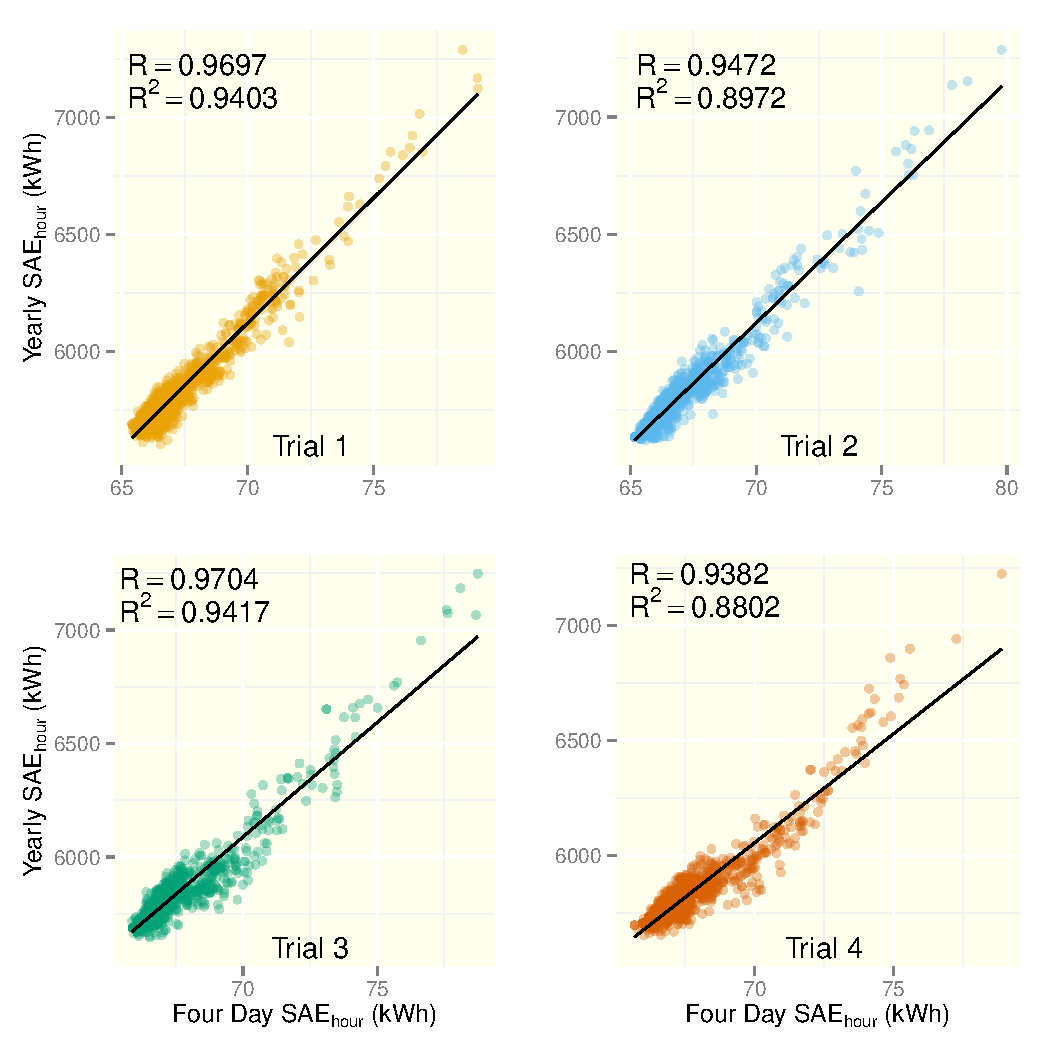
\includegraphics[width=5in]{figure1}
\caption{Each of the four independent trials show very high correlation between four-day and full-year-schedule SAE of hourly electrical usage. This means that an abbreviated surrogate (four-day schedule) is a plausible method of expediting the tuning.}
\label{fig:hour-corr}
\end{figure}

\begin{table}[tbp]
\centering
\caption{The sampling of the SAE to determine correlation was done using an evolutionary computation with the objective of minimizing the SAE. This produced initial samples with relatively high SAE values and subsequent samples with generally lower SAE as more data was used. The correlation using only the first $N$\% of the samples produced shows that even the initial samples have strong correlation most of the time (with the exception of Trial 3).}
\label{tab:hour-corr}
\begin{tabular}{ccccc}
\toprule
Data Used & Trial 1 & Trial 2 & Trial 3 & Trial 4\\
\midrule
100\% & 0.9603 & 0.9422 & 0.9015 & 0.9555\\\rowcolor{DarkRow}
90\%  & 0.8668 & 0.8438 & 0.6545 & 0.8788\\
80\%  & 0.8683 & 0.8573 & 0.6444 & 0.8922\\\rowcolor{DarkRow}
70\%  & 0.8726 & 0.8561 & 0.6231 & 0.8944\\
60\%  & 0.8671 & 0.8489 & 0.6078 & 0.8952\\\rowcolor{DarkRow}
50\%  & 0.8703 & 0.8489 & 0.5557 & 0.8971\\
40\%  & 0.8774 & 0.8417 & 0.5663 & 0.9020\\\rowcolor{DarkRow}
30\%  & 0.8794 & 0.8208 & 0.6015 & 0.8973\\
20\%  & 0.8841 & 0.8231 & 0.5988 & 0.8860\\\rowcolor{DarkRow}
10\%  & 0.8796 & 0.8235 & 0.3985 & 0.8714\\
\bottomrule
\end{tabular}
\end{table}


\subsection{Experiment 2---Tuning Using the Abbreviated Schedule}
\label{sub:experiment2}
The abbreviated schedule is desirable since it is significantly less expensive to compute, has been shown an effective surrogate for full-schedule error, and provides a baseline to which other results can be compared and contextualized. In Experiment 2, we tune the refined and primitive models on hourly electrical usage with the abbreviated schedule. We then use the four-day tuned models to calculate data for the entire year in order to get a full-schedule SAE that is directly comparable to other experiments.

Table~\ref{tab:hourly-abbrev} presents the final population statistics for full-schedule SAE on each model and trial. In this table, the actual full-schedule data was compared to each of the 16 candidates in the final population for each trial, and the average and minimum SAE values from this comparison are reported. For the refined model, the average minimum yearly SAE achieved by the EC was 5,660 kWh. This corresponds to a reduction of 582 kWh in SAE, which is an almost 10\% reduction from the model, which had an SAE of 6,242 kWh. For the primitive model, the average minimum yearly SAE was 7,453 kWh, which is a reduction of 660 kWh or an 8\% reduction in SAE. This is also a 35\% reduction of the error between the primitive and refined models (8,114 kWh for the primitive and 6,242 kWh for the refined).


\begin{table}[tbp]
\centering
\caption{In Experiment 2, the evolutionary computation was used to optimize the primitive and refined models eight independent times (thus, 16 different tunings) using the abbreviated schedule. The final population of 16 individuals for each tuning were used to produce the statistics in this table. The average and minimum $SAE_{hour}$ (kWh) values for electrical usage from the final populations are shown.}
\label{tab:hourly-abbrev}
\begin{tabular}{llcccccccc}
\toprule
 &  & \multicolumn{8}{c}{Trial (kWh)}\\
Model & Metric & 1 & 2 & 3 & 4 & 5 & 6 & 7 & 8\\
\midrule
Primitive & Avg & 7539 & 7578 & 7683 & 7638 & 7495 & 7467 & 7503 & 7587\\\rowcolor{DarkRow}
Refined   & Avg & 5720 & 5708 & 5792 & 5762 & 5750 & 5783 & 5806 & 5698\\
Primitive & Min & 7393 & 7507 & 7595 & 7545 & 7393 & 7360 & 7356 & 7477\\\rowcolor{DarkRow}
Refined   & Min & 5620 & 5625 & 5709 & 5687 & 5640 & 5671 & 5711 & 5616\\
\bottomrule
\end{tabular}
\end{table}


\subsection{Experiment 3---Tuning Using the Full Schedule}
\label{sub:experiment3}
As a means of comparison, this experiment focuses on using the full schedule for tuning the models. This approach is more computationally expensive than using the abbreviated schedule. The only difference between this experiment and Experiment 2 is the use of the full schedule for the EnergyPlus simulation for calculating candidate fitness. The expectation is that this would generate tuned models with lower SAE values when compared against actual data.

Table~\ref{tab:hourly-full} displays the final population statistics for the full-schedule SAE on each model and trial. As in Table~\ref{tab:hourly-abbrev}, these statistics are the population averages and minimums. For the refined model, the average minimum SAE across eight trials was 5,539 kWh. Compare this error to that of the baseline file (6,242 kWh) and of the abbreviated schedule EC (5,660 kWh). Clearly, using the full schedule throughout the evolution provides a lower error (by 121 kWh) than using the abbreviated schedule. However, this additional 2\% reduction in error beyond that of the abbreviated schedule requires more than five times the computational resources. The abbreviated-schedule EC was able to complete a single trial in about 1.5 hours on an eight-core machine, whereas the full schedule EC required 8 hours on the same machine. For the primitive model, the average minimum SAE across eight trials was 7,162 kWh. Once again, this error must be compared to the baseline file (8,114 kWh) and to the abbreviated-schedule EC (7,453 kWh). Here, there is a reduction of 291 kWh in SAE from the abbreviated schedule, which corresponds to a 4\% reduction for a similar five-fold increase in computational time.

\begin{table}[tbp]
\centering
\caption{In Experiment 3, the evolutionary computation was used to optimize the primitive and refined models eight independent times (thus, 16 different tunings) using the full schedule. The final population of 16 individuals for each tuning were used to produce the statistics in this table. The average and minimum $SAE_{hour}$ (kWh) values for electrical usage from the final populations are shown.}
\label{tab:hourly-full}
\begin{tabular}{llcccccccc}
\toprule
 &  & \multicolumn{8}{c}{Trial (kWh)}\\
Model & Metric & 1 & 2 & 3 & 4 & 5 & 6 & 7 & 8\\
\midrule
Primitive & Avg & 7275 & 7245 & 7250 & 7259 & 7338 & 7202 & 7274 & 7272\\\rowcolor{DarkRow}
Refined   & Avg & 5582 & 5641 & 5620 & 5594 & 5636 & 5623 & 5623 & 5596\\
Primitive & Min & 7175 & 7138 & 7150 & 7122 & 7253 & 7114 & 7162 & 7179\\\rowcolor{DarkRow}
Refined   & Min & 5518 & 5568 & 5527 & 5510 & 5560 & 5550 & 5558 & 5523\\
\bottomrule
\end{tabular}
\end{table}



\subsection{Experiment 4---Tuning Using Both Schedules Serially}
\label{sub:experiment4}
As shown in Experiment 3, the full schedule produces better tuning results but requires more computational resources. If additional resources are allotted, it may be best to employ those after the tuning process has produced a set of faithful models. The evolutionary computation can be started from a known set of good solutions (which we call \emph{seeds}), and that allows us to tune in two parts---first with the abbreviated schedule to produce a set of seeds and then with the full schedule to produce the final tuning.

In this experiment, the first 768 E+ simulations were done using the four-day schedule. At the end of those simulations, the best half (8) of the final population's candidate solutions were inserted as seeds into a new initial population of 16 candidates. (The other 8 candidates were randomly generated.) This population was then evolved for the remaining 256 evaluations on the yearly schedule.

Table~\ref{tab:hourly-serial} shows the final population minimums and averages for each trial for both the refined and primitive models. The average minimum SAE for the refined model was 5,581 kWh, and for the primitive model it was 7,343 kWh. As expected, the performance is better than using the abbreviated schedule alone (5,660 kWh and 7,453 kWh for refined and primitive models, respectively), but it is not as good as using the full schedule throughout the evolution (5,539 kWh and 7,162 kWh). The reduction in SAE was 79 kWh for the refined model and 110 kWh for the primitive model, which corresponds to a movement of 66\% and 38\% toward the full schedule performance for each model. This performance comes at a cost of approximately double the computational expense of the abbreviated schedule only (3 hours instead of 1.5 hours), which is less than the five-times-increase of the full schedule (over 8 hours). 


\begin{table}[tbp]
\centering
\caption{In Experiment 4, the evolutionary computation was used to optimize the primitive and refined models eight independent times (thus, 16 different tunings) using the abbreviated schedule for the first 75\% of the evaluations and the full schedule for the remaining 25\%. The final population of 16 individuals for each tuning were used to produce the statistics in this table. The average and minimum $SAE_{hour}$ (kWh) values for electrical usage from the final populations are shown.}
\label{tab:hourly-serial}
\begin{tabular}{llcccccccc}
\toprule
 &  & \multicolumn{8}{c}{Trial (kWh)}\\
Model & Metric & 1 & 2 & 3 & 4 & 5 & 6 & 7 & 8\\
\midrule
Primitive & Avg & 7404 & 7463 & 7469 & 7467 & 7393 & 7381 & 7434 & 7403\\\rowcolor{DarkRow}
Refined   & Avg & 5626 & 5670 & 5688 & 5614 & 5695 & 5667 & 5642 & 5646\\
Primitive & Min & 7306 & 7382 & 7402 & 7378 & 7328 & 7283 & 7362 & 7306\\\rowcolor{DarkRow}
Refined   & Min & 5564 & 5586 & 5608 & 5545 & 5596 & 5618 & 5566 & 5563\\
\bottomrule
\end{tabular}
\end{table}

\subsection{Experiment 5---Tuning Using Both Schedules in Parallel}
\label{sub:experiment5}
Rather than executing the different evolutionary approaches in serial fashion, it is possible to perform them in parallel using an island-model EC \cite{cit:eiben2007}. In this experiment, two different populations of 16 candidate solutions are maintained. The first (``fast'') island uses the abbreviated schedule for simulation, and the second (``slow'') uses the full-year schedule. At the end of each generation (i.e., each 16 simulations), a one-element migration queue is queried for any existing candidate. If one is found, it replaces the worst candidate in the population. In either case, the best candidate in the population is inserted into the queue. Since both populations perform this migration, this enables solutions to transfer between the populations (or ``islands''). Note that that all immigrant solutions are re-evaluated to determine the fitness under the new simulation approach before they are inserted into the population.

Table~\ref{tab:hourly-parallel} shows the final population statistics for the candidates from the abbreviated-schedule islands for both primitive and refined models. The average minimum SAE was 5,597 kWh for the refined model and 7,270 kWh for the primitive model. This is very near the performance obtained from the serial evolution. However, the parallel approach has a number of advantages. First, and perhaps most importantly, it makes no assumptions about the number of simulations that will be carried out, so users are free to stop the tuning process at any time. Since the full simulation is always being run on one of the islands, this information is always incorporated in the final population. Second, the parallel approach appears to provide slightly better performance in terms of the SAE-to-full-year-simulation ratio. This is because the actual performance between the two is nearly identical, but the parallel version's full island was unable to make use of particularly good solutions from the abbreviated island until after about the first 25\% of simulations had been run. So, in some sense, it achieved similar error performance using only 75\% of the simulations. This 25\% is an estimate based on the typical convergence of the abbreviated island as shown in Figure~\ref{fig:hour-converge}. This figure plots the convergence of the error of the best refined-model candidate through each generation for each trial of Experiment 4 (up through generation 48, after which the full-schedule information was used). Generation 12 represents the 25\% mark (shown as a dotted line in the figure) of the full 1,024 evaluations.

\begin{table}[tbp]
\centering
\caption{In Experiment 5, an island-model evolutionary computation was used to optimize the primitive and refined models eight independent times (thus, 16 different tunings) using a \emph{slow} and a \emph{fast} island. The final population of 16 individuals for each tuning were used to produce the statistics in this table. The average and minimum $SAE_{hour}$ (kWh) values for electrical usage from the final populations are shown.}
\label{tab:hourly-parallel}
\begin{tabular}{llcccccccc}
\toprule
 &  & \multicolumn{8}{c}{Trial (kWh)}\\
Model & Metric & 1 & 2 & 3 & 4 & 5 & 6 & 7 & 8\\
\midrule
Primitive & Avg & 7340 & 7330 & 7435 & 7470 & 7391 & 7349 & 7390 & 7356\\\rowcolor{DarkRow}
Refined   & Avg & 5724 & 5675 & 5670 & 5660 & 5648 & 5715 & 5669 & 5625\\
Primitive & Min & 7218 & 7201 & 7360 & 7373 & 7281 & 7211 & 7293 & 7226\\\rowcolor{DarkRow}
Refined   & Min & 5639 & 5597 & 5582 & 5578 & 5580 & 5633 & 5591 & 5573\\
\bottomrule
\end{tabular}
\end{table}

\begin{figure}[tbp]
\centering
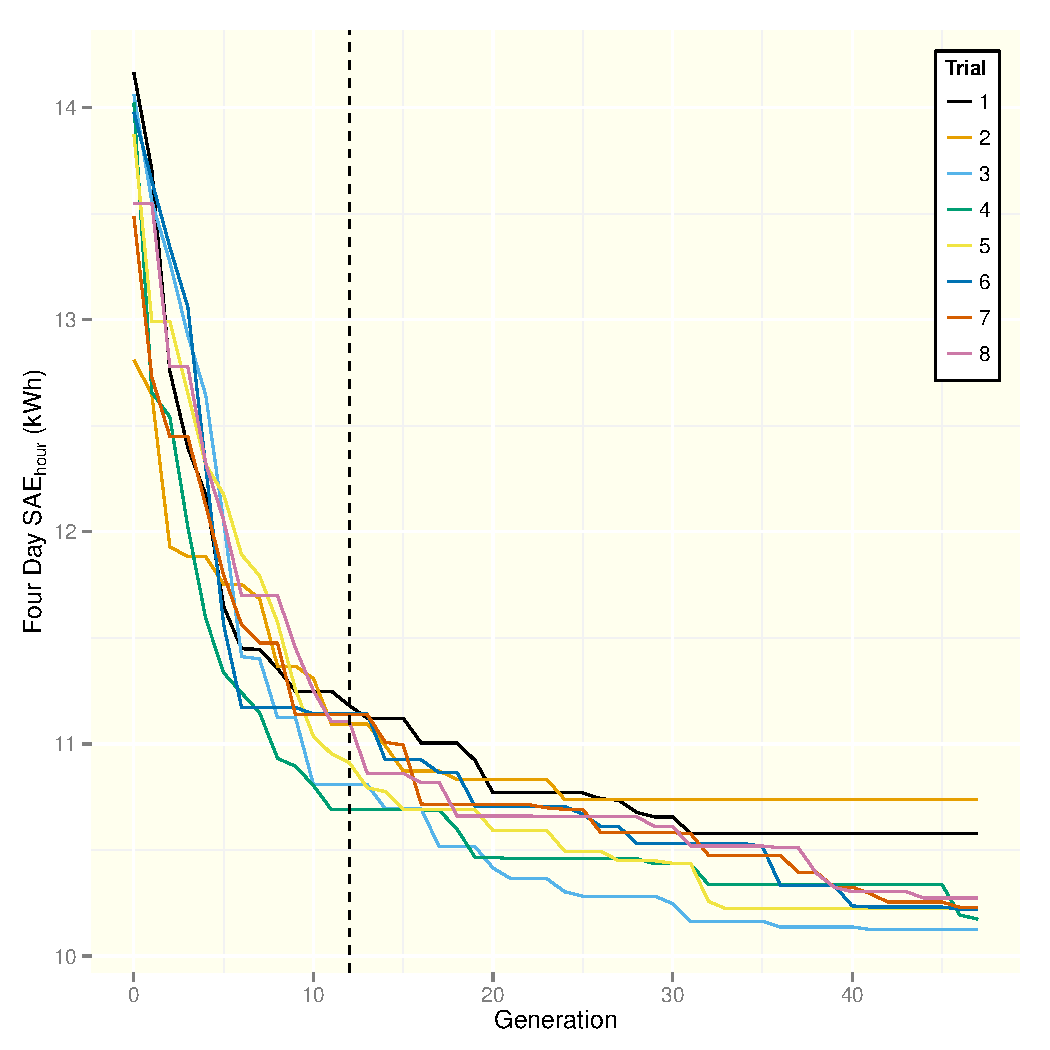
\includegraphics[width=5in]{figure2}
\caption{This figure shows the convergence of the best individual in each trial of Experiment 4 when using the abbreviated schedule (i.e., the first 75\% of the evaluations). The dotted line marks generation 12, which is 25\% of the evaluations allotted to the abbreviated schedule. Prior to this point, individuals produced by the abbreviated schedule tuning are not particularly useful as seeds due to their relatively high SAE. After this point, they become much more useful.}
\label{fig:hour-converge}
\end{figure}


\section{Conclusions and Future Work}
\label{sec:conclusions}
The results of the previous experiments are summarized in Table~\ref{tab:hourly-summary} and Figure~\ref{fig:hourly-summary}. This table shows the baseline and various approaches for tuning for each model, focusing on the SAE and RMSE between the model output and the actual data. The percentages in parentheses are the percent reduction in error from the baseline.

These experiments have shown that it is possible to use an evolutionary search to reduce the RMSE by over 7\% when comparing hourly electrical usage. They have also shown that a two-island approach is both a feasible and effective way of combining the abbreviated- and full-schedule approaches. 

Experiment 1 verified that a four-day schedule could serve as a viable surrogate for the full-year schedule in terms of hourly electrical usage, producing a correlation coefficient of 0.96 between abbreviated and full schedules. Experiment 2 showed that an abbreviated-only approach was able to reduce the RMSE by 6\% and 7\% below the baseline for the refined and primitive models, respectively. Experiment 3 focused on using the full schedule only, and that approach reduced the RMSE by 7\% (refined) and 10\% (primitive). Experiment 4 combined the two approaches in serial fashion, using the abbreviated schedule for the first 768 simulations and then using the full schedule for the remaining 256. This approach was better than the abbreviated schedule alone, but it performed only slightly worse than the full schedule alone. Finally, Experiment 5 combined the two approaches in parallel using an island model, where one island used the abbreviated schedule and the other used the full schedule. Solutions were able to migrate between the islands, and this approach was competitive with the full schedule approach, despite the fact that it only used 25\% of the full-schedule simulations.


\begin{table}[tbp]
\centering
\caption{The summary comparison of results from Experiments 2--5 show that significant reduction can be gained from tuning with an abbreviated schedule, either alone, serially, or in parallel with a full-schedule tuning. Percentages in parentheses are reductions versus the baseline.}
\label{tab:hourly-summary}
\begin{tabular}{lllll}
\toprule
 &  \multicolumn{2}{c}{Refined} & \multicolumn{2}{c}{Primitive}\\
Approach & SAE (kWh) & RMSE & SAE (kWh) & RMSE \\
\midrule
Baseline    & 6242        & 1.206       & 8114        & 1.625 \\\rowcolor{DarkRow}
Abbreviated & 5660 (9\%)  & 1.129 (6\%) & 7453 (8\%)  & 1.514 (7\%)\\
Full        & 5539 (11\%) & 1.119 (7\%) & 7162 (12\%) & 1.458 (10\%)\\\rowcolor{DarkRow}
Serial      & 5581 (11\%) & 1.123 (7\%) & 7343 (9\%)  & 1.497 (8\%)\\
Parallel    & 5597 (10\%) & 1.121 (7\%) & 7270 (10\%) & 1.482 (9\%)\\
\bottomrule
\end{tabular}
\end{table}

\begin{figure}[tbp]
\centering
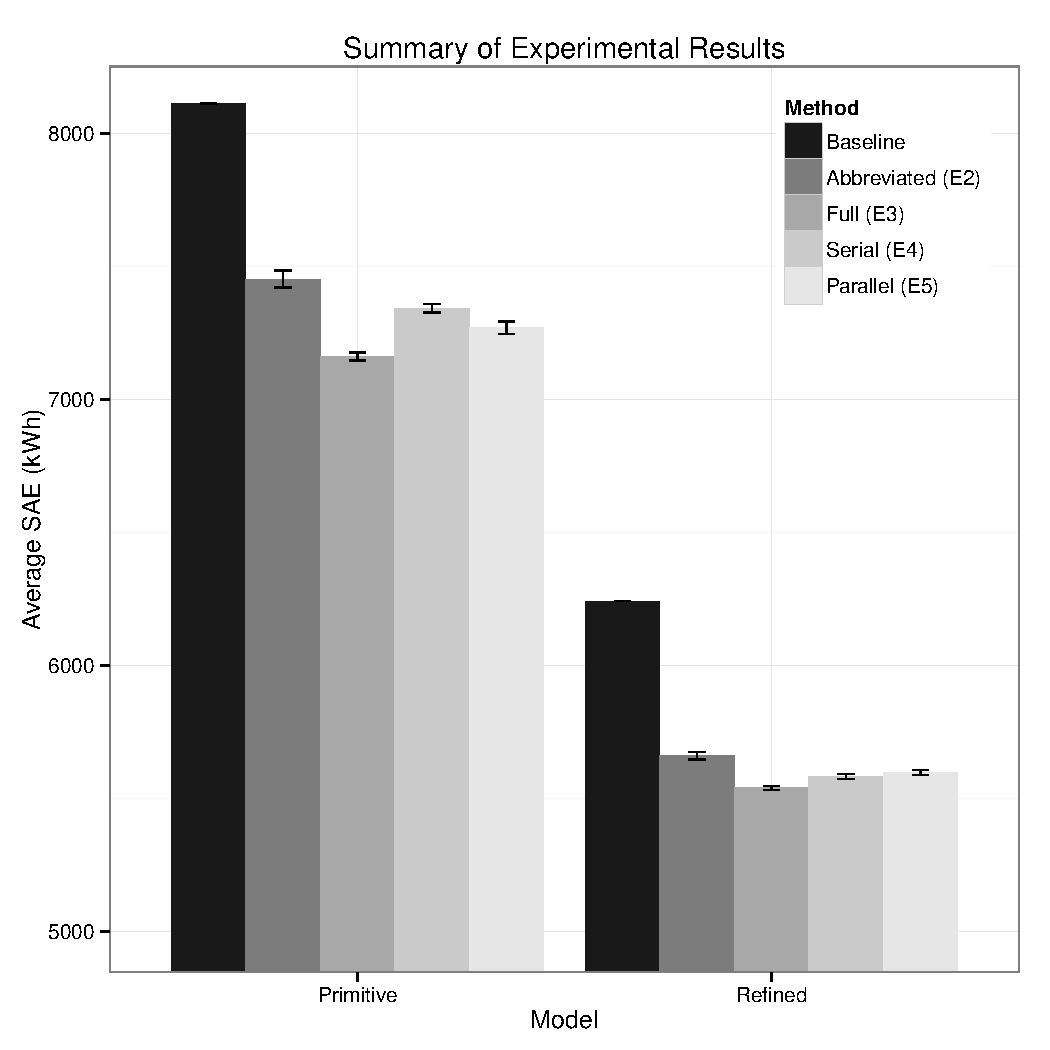
\includegraphics[width=5in]{figure3}
\caption{This figure shows the results of Experiments 2--5 when compared to the baseline (see Table~\ref{tab:hourly-summary}). The average minimum SAE value found across all eight trials is used to represent each method, and each method is accompanied by standard error bars (except for the baseline). The y-axis minimum value was increased to 5,000 in order to highlight the differences between the methods.}
\label{fig:hourly-summary}
\end{figure}

In conclusion, we've shown a series of experiments which elucidate several methods, advantages, and trade-offs when using evolutionary computation for automatically calibrating a software model of an emulated-occupancy experimental residential building to hourly whole-building electrical data. Work is ongoing to extend these methods for calibration to residential buildings where fewer things are certain, to larger commercial buildings, calibrating to sub-hourly data for multiple data channels, and quantitative tests for determining not only how close the building matches measured data but also how accurately the tuned model matches the real building.


\section{Acknowledgements}
This work was funded by field work proposal CEBT105 under the Department of Energy Building Technology Activity Number BT0201000. We would like to thank Amir Roth for his support and review of this project. This research used resources of the Oak Ridge Leadership Computing Facility at the Oak Ridge National Laboratory, which is supported by the Office of Science of the U.S. Department of Energy under Contract No. DE-AC05-00OR22725. Our work has been enabled and supported by data analysis and visualization experts at the RDAV (Remote Data Analysis and Visualization) Center of the University of Tennessee, Knoxville (NSF grant no. ARRA-NSF-OCI-0906324 and NSF-OCI-1136246). Oak Ridge National Laboratory is managed by UT-Battelle, LLC, for the U.S. Dept. of Energy under contract DE-AC05-00OR22725. This manuscript has been authored by UT-Battelle, LLC, under Contract Number DEAC05-00OR22725 with the U.S. Department of Energy. The United States Government retains and the publisher, by accepting the article for publication, acknowledges that the United States Government retains a non-exclusive, paid-up, irrevocable, world-wide license to publish or reproduce the published form of this manuscript, or allow others to do so, for United States Government purposes.


%% The Appendices part is started with the command \appendix;
%% appendix sections are then done as normal sections
%% \appendix

%% \section{}
%% \label{}

%% References
%%
%% Following citation commands can be used in the body text:
%% Usage of \cite is as follows:
%%   \cite{key}          ==>>  [#]
%%   \cite[chap. 2]{key} ==>>  [#, chap. 2]
%%   \citet{key}         ==>>  Author [#]

%% References with bibTeX database:

\bibliographystyle{model1-num-names}
\bibliography{autotune}

%% Authors are advised to submit their bibtex database files. They are
%% requested to list a bibtex style file in the manuscript if they do
%% not want to use model1a-num-names.bst.

%% References without bibTeX database:

% \begin{thebibliography}{00}

%% \bibitem must have the following form:
%%   \bibitem{key}...
%%

% \bibitem{}

% \end{thebibliography}


\end{document}

%%
%% End of file `elsarticle-template-1a-num.tex'.
